\documentclass[a4paper,12pt,twoside]{article}
\usepackage{graphicx}
\graphicspath{ {./images/} }
\usepackage{wrapfig}
%\usepackage{indentfirst} % Uncomment to indent first paragraph of each section (not really correct for academic papers, but follows more common business convention)

\usepackage{subcaption} 

\usepackage{geometry}
\geometry{
  a4paper,
  total={170mm,257mm},
  left=20mm,
  top=40mm,
  bottom=30mm,
}

\usepackage{fontspec}
\setmainfont{Exo 2}[%
    Path            =   fonts/,
    Extension       =   .otf,
    UprightFont     =   *-Regular,
    ItalicFont      =   *-Italic,
    BoldFont        =   *-Bold,
    BoldItalicFont  =   *-BoldItalic,
    FontFace        =   {black}{n}{*-Black},
    FontFace        =   {black}{it}{*-BlackItalic},
]

\usepackage[dvipsnames]{xcolor}
\definecolor{RHgrey}{RGB}{101,101,101}
\definecolor{RHblue}{RGB}{7,163,216}
\definecolor{RHgreen}{RGB}{30,165,43}
\definecolor{RHyellow}{RGB}{251,210,0}
\definecolor{code}{RGB}{200,200,200}
\definecolor{textbox}{RGB}{200,255,200}
  
\usepackage{sectsty}
\sectionfont{\color{RHblue}} 
\subsectionfont{\color{RHblue}}
\subsubsectionfont{\color{RHblue}}

\usepackage[utf8]{inputenc}
\usepackage[english]{babel}

\usepackage{multicol} % Allows multiple columns to be used on the fly

\usepackage{fancyhdr}
\pagestyle{fancy}
\fancyhf{}
\lhead{\color{RHgrey} \leftmark}
\rhead{\color{RHgrey} \rightmark}
\fancyfoot[LE]{\color{RHgrey} \thepage \hspace{5mm} \scriptsize RAMANI HURIA INTERIM REPORT 4}
\fancyfoot[RO]{\color{RHgrey} \scriptsize RAMANI HURIA INTERIM REPORT 4 \hspace{3mm} \normalsize \thepage}

\usepackage{hyperref}
\hypersetup{
  colorlinks=true,
  linkcolor=RHblue, % to match the Ramani Huria blue text
  filecolor=magenta,      
  urlcolor=cyan,
  pdftitle={RH Interim Report 4},
  bookmarks=true,
  %pdfpagemode=FullScreen,
}
%\urlstyle{same}

\usepackage[framemethod=tikz]{mdframed}
\usepackage{lipsum}


\title{Ramani Huria Interim Report 4}
\author{Humanitarian OpenStreetMap Team}
\usepackage[nodayofweek,level]{datetime}
\newdate{date}{15}{04}{2019}
\date{\displaydate{date}}

\newcommand*{\vcenteredhbox}[1]{\begingroup
\setbox0=\hbox{#1}\parbox{\wd0}{\box0}\endgroup} % For creating vertically centered rows of logos

\setcounter{tocdepth}{2} % Table of Contents includes only sections and subsections, not subsubsections.

\begin{document}
\thispagestyle{empty}
\begin{center}
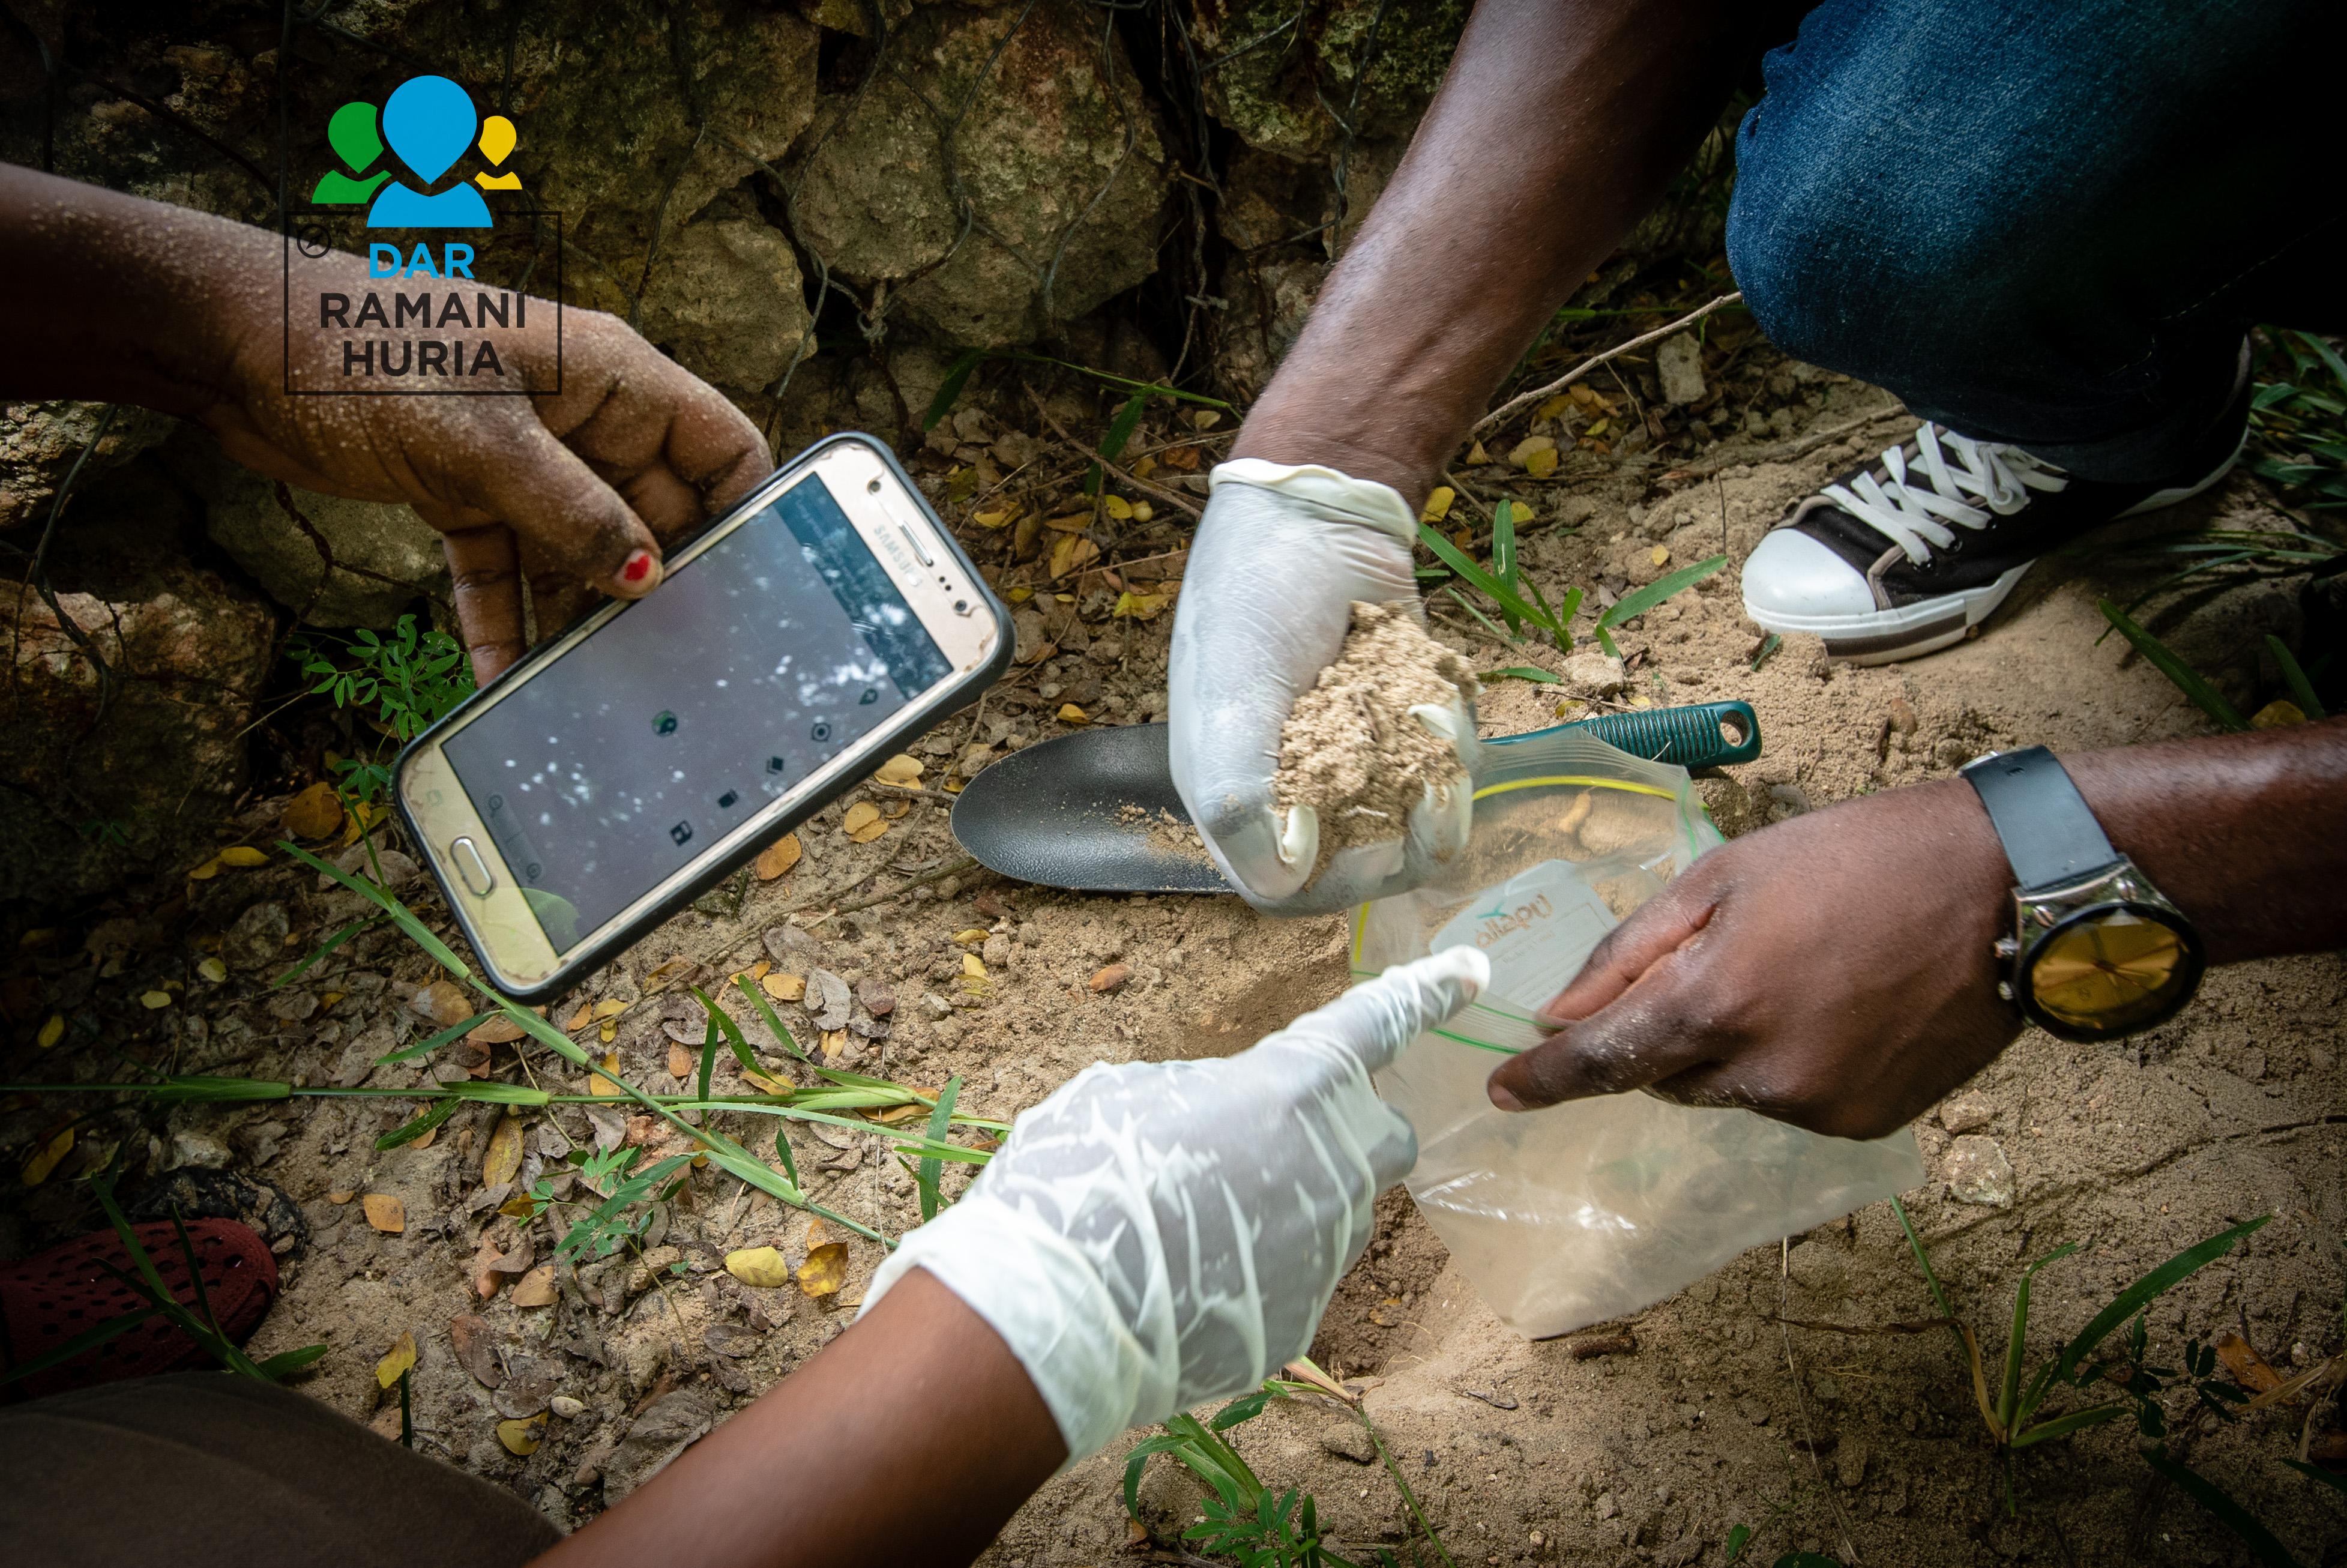
\includegraphics[width=\textwidth]{Cover_photo_with_logo.jpg}
\end{center}
\bigskip
\begin{center}
  \Huge \color{RHblue} \textbf {RAMANI HURIA}

\textbf{INTERIM REPORT 4}
\end{center}
\bigskip
\vbox{
  \centering
  Prepared for:
  \vcenteredhbox{
\includegraphics[width=2cm]{UK-aid_logo.png}}
  and { }
  \vcenteredhbox{
\includegraphics[width=7cm]{images/World_Bank_Group_logo.png}}
  \
  
  by:
  \vcenteredhbox{
\includegraphics[width=4cm]{HOT_logo_with_text.png}}
  % \maketitle
  
}
\medskip
\begin{center}
  Humanitarian OpenStreetMap
  \
  
  15 April, 2019
\end{center}
\bigskip
\bigskip
\bigskip
\begin{center}
\color{RHblue}\rule{\textwidth}{0.6cm}
\end{center}

\newpage
\color{RHgrey}

\begin{center}
{
\includegraphics[width=5cm]{Dar_Ramani_Huria_logo.png}}
\end{center}

This report was prepared by William Evans, Innocent Maholi, Ivan Buendia Gayton, and \textcolor{red}{OTHER PEOPLE} from the Humanitarian OpenStreetMap Team in Tanzania.

\medskip

Layout and graphic design by Ivan Buendia Gayton based on the Ramani Huria design guideline by Darragh Amelia Coward, using the the \LaTeX { } typesetting system.

\medskip

Guidance and input on the project came from Edward Anderson, Caroline Gevaert, Roza Vasileva, and Msilikale Msilanga at the World Bank.

\medskip

Unless otherwise noted, photos by the Ramani Huria team.
5
 Maps were prepared by the Ramani Huria team using QGIS.

\bigskip\bigskip

\textcolor{red}{LOTS OF LOGOS}

\newpage

\tableofcontents

\newpage
\section{Executive Summary}
\label{executivesummary}
\begin{multicols}{2}

  \begin{mdframed}[hidealllines=true,backgroundcolor=RHgreen!10,innerleftmargin=6pt,innerrightmargin=6pt,leftmargin=-3pt,rightmargin=-3pt]

\color{RHgrey}
    
With the support of the World Bank in Tanzania, the Ramani Huria (RH) team has been collecting data for urban resilience with a particular emphasis on flooding since 2015. As the program nears its end in September of 2019, the RH team is now primarily working to curate, organize, document, and publish the data, tools and knowledge that have been created. 

We are working to transfer knowledge and hand over to Tanzania Resilience Academy, the successor project to Ramani Huria. 
\end{mdframed}

Together with the coalescing Resilience Academy team, we are working to disseminate the knowledge and data to as many users---particularly those who are likely to have impact improving resilience---as possible. 

I want this report to get 100\% marks.

\lipsum[10-18]

\end{multicols}

%\includegraphics[width=0.8\textwidth]{sample_locations.jpg}

\newpage
\section{Introduction}
\label{Introduction}

This report will tell you about stuff

\begin{itemize}
  \item Like this
  \item And this
\end{itemize}

We also would like to point out a link to  \href{https://ramanihuria.org}{a website}\footnote{\url{http://ramanihuria.org}\color{RHgrey} { }because it's really, really interesting. You should click on that link.}. Did you notice that there was a footnote there? If you look at the footnote it contains the full URL of the link, so that people reading the document on paper can see what it links to? Cool, huh? The rest of the text on this page will be in two columns, just because we can do that with the \LaTeX{} \textbf{\textit{multicols}} plugin. By the way, I can highlight code with a color box like \textbf{\colorbox{code}{this.}}

\begin{multicols}{2}

  \lipsum[5-8]
  
\end{multicols}

\newpage
\section{Monthly Activity Summary}

The graphic below shows all the stuff we did in each month! Wow!

\bigskip

\begin{itemize}
    \item October 2018
Drainage Mapping
Hyper-local administrative boundary mapping
Soil sampling
Tabata Trash Mapping
    \item November 2018
Hyper-local administrative boundary mapping
Soil sampling
Tabata Trash Mapping
    \item December 2018
Hyper-local administrative boundary mapping
Soil sampling
Tabata Trash Mapping
Asset and Threat Mapping
Data publication on GeoNode with Uhurulabs
    \item January 2019
Drainage mapping
Tabata Trash Mapping
Asset and Threat Mapping
    \item February 2019
Soil sampling
Tabata Trash Mapping
Drainage Mapping
Asset and Threat Maps Production
Data Quality Assurance
Data publication on GeoNode with Uhurulabs
\end{itemize}

\section{Team Composition and Assignments}
Hi there!

\section{Data Quality}
This is the data quality process. 

We do the following steps


\section{Datasets}

\subsection{Drainage}
\begin{wrapfigure}{r}{0.25\textwidth} %this figure will be at the right
    \centering
    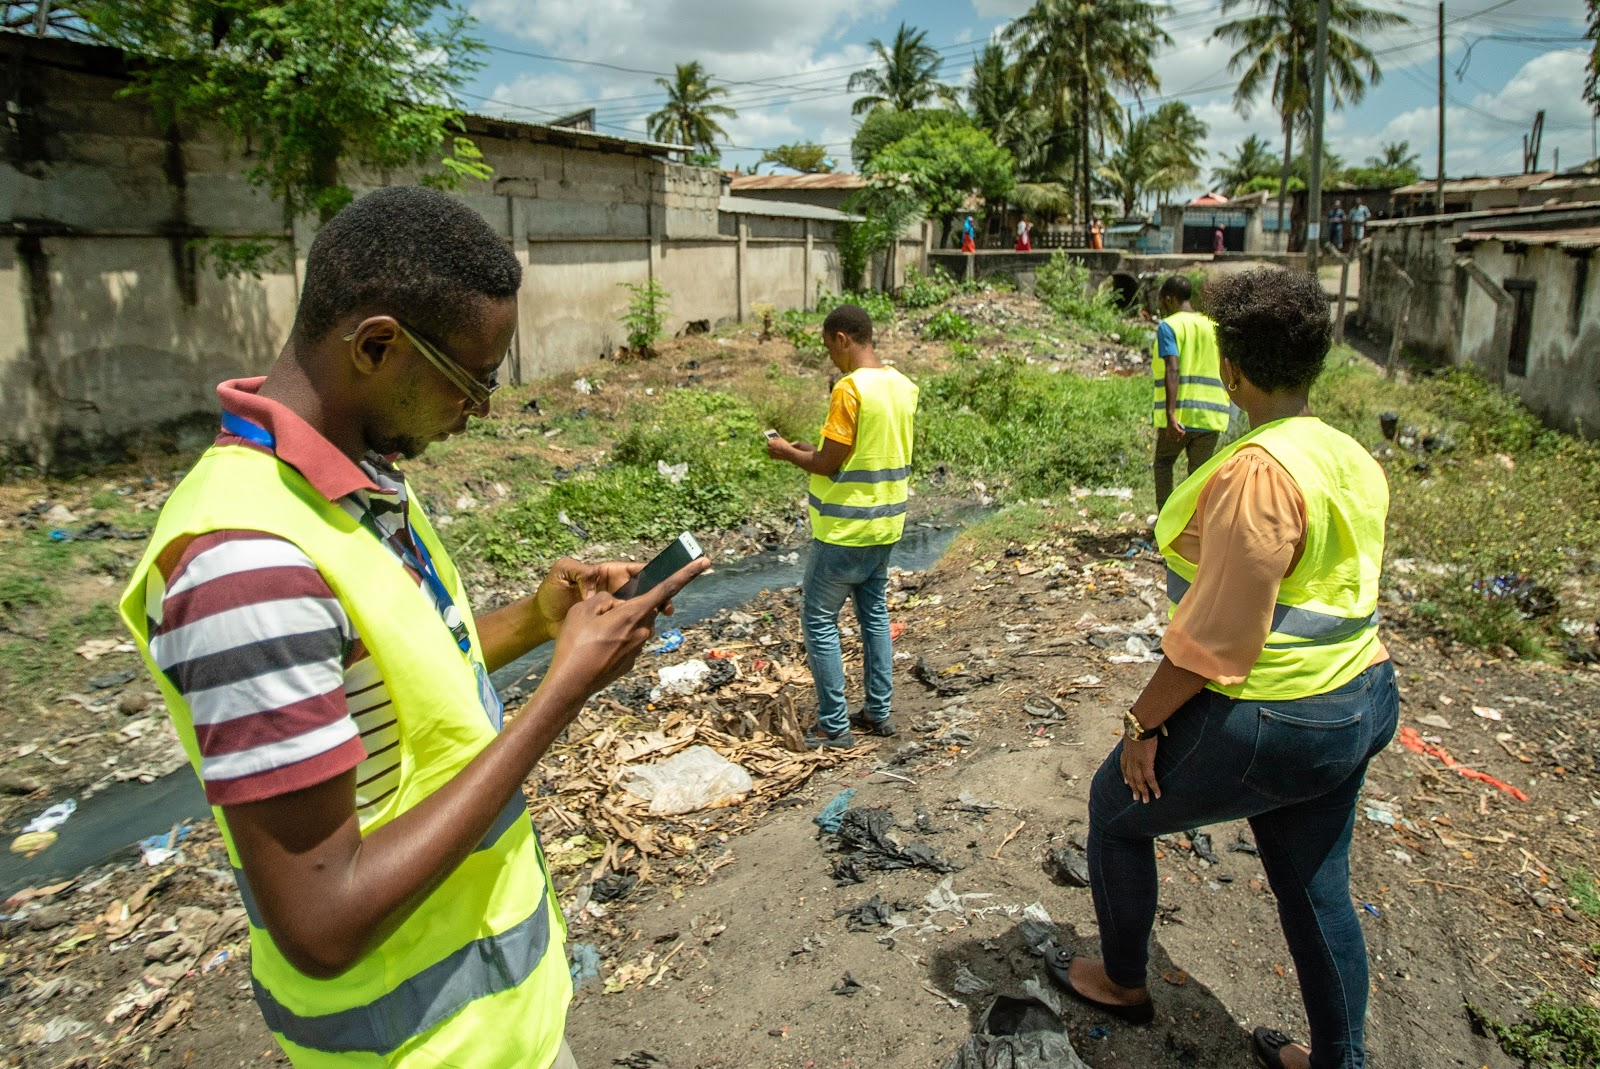
\includegraphics[width=0.25\textwidth]{images/Drainage_Mapping.jpg}
\end{wrapfigure}

\

Drainage data collected in the most flood prone areas across Dar es Salaam using cheap  and practical methods. This information will be used to develop a flood model which requires accurately collected specifications of drains such as depth, width, blockage (by either vegetation or material), connectivity, and diameter (typically for culverts).

\subsubsection{Spatial Extent}
Drainage data covers 44 prioritized Ramani Huria wards most of which are along the Msimbazi and Ng’ombe rivers. Almost 90\% of the wards have been mapped.

\begin{figure}[h]
  \color{RHgreen}\caption{Map showing the drainage mapping progress as of March, 2019}
  \centering
  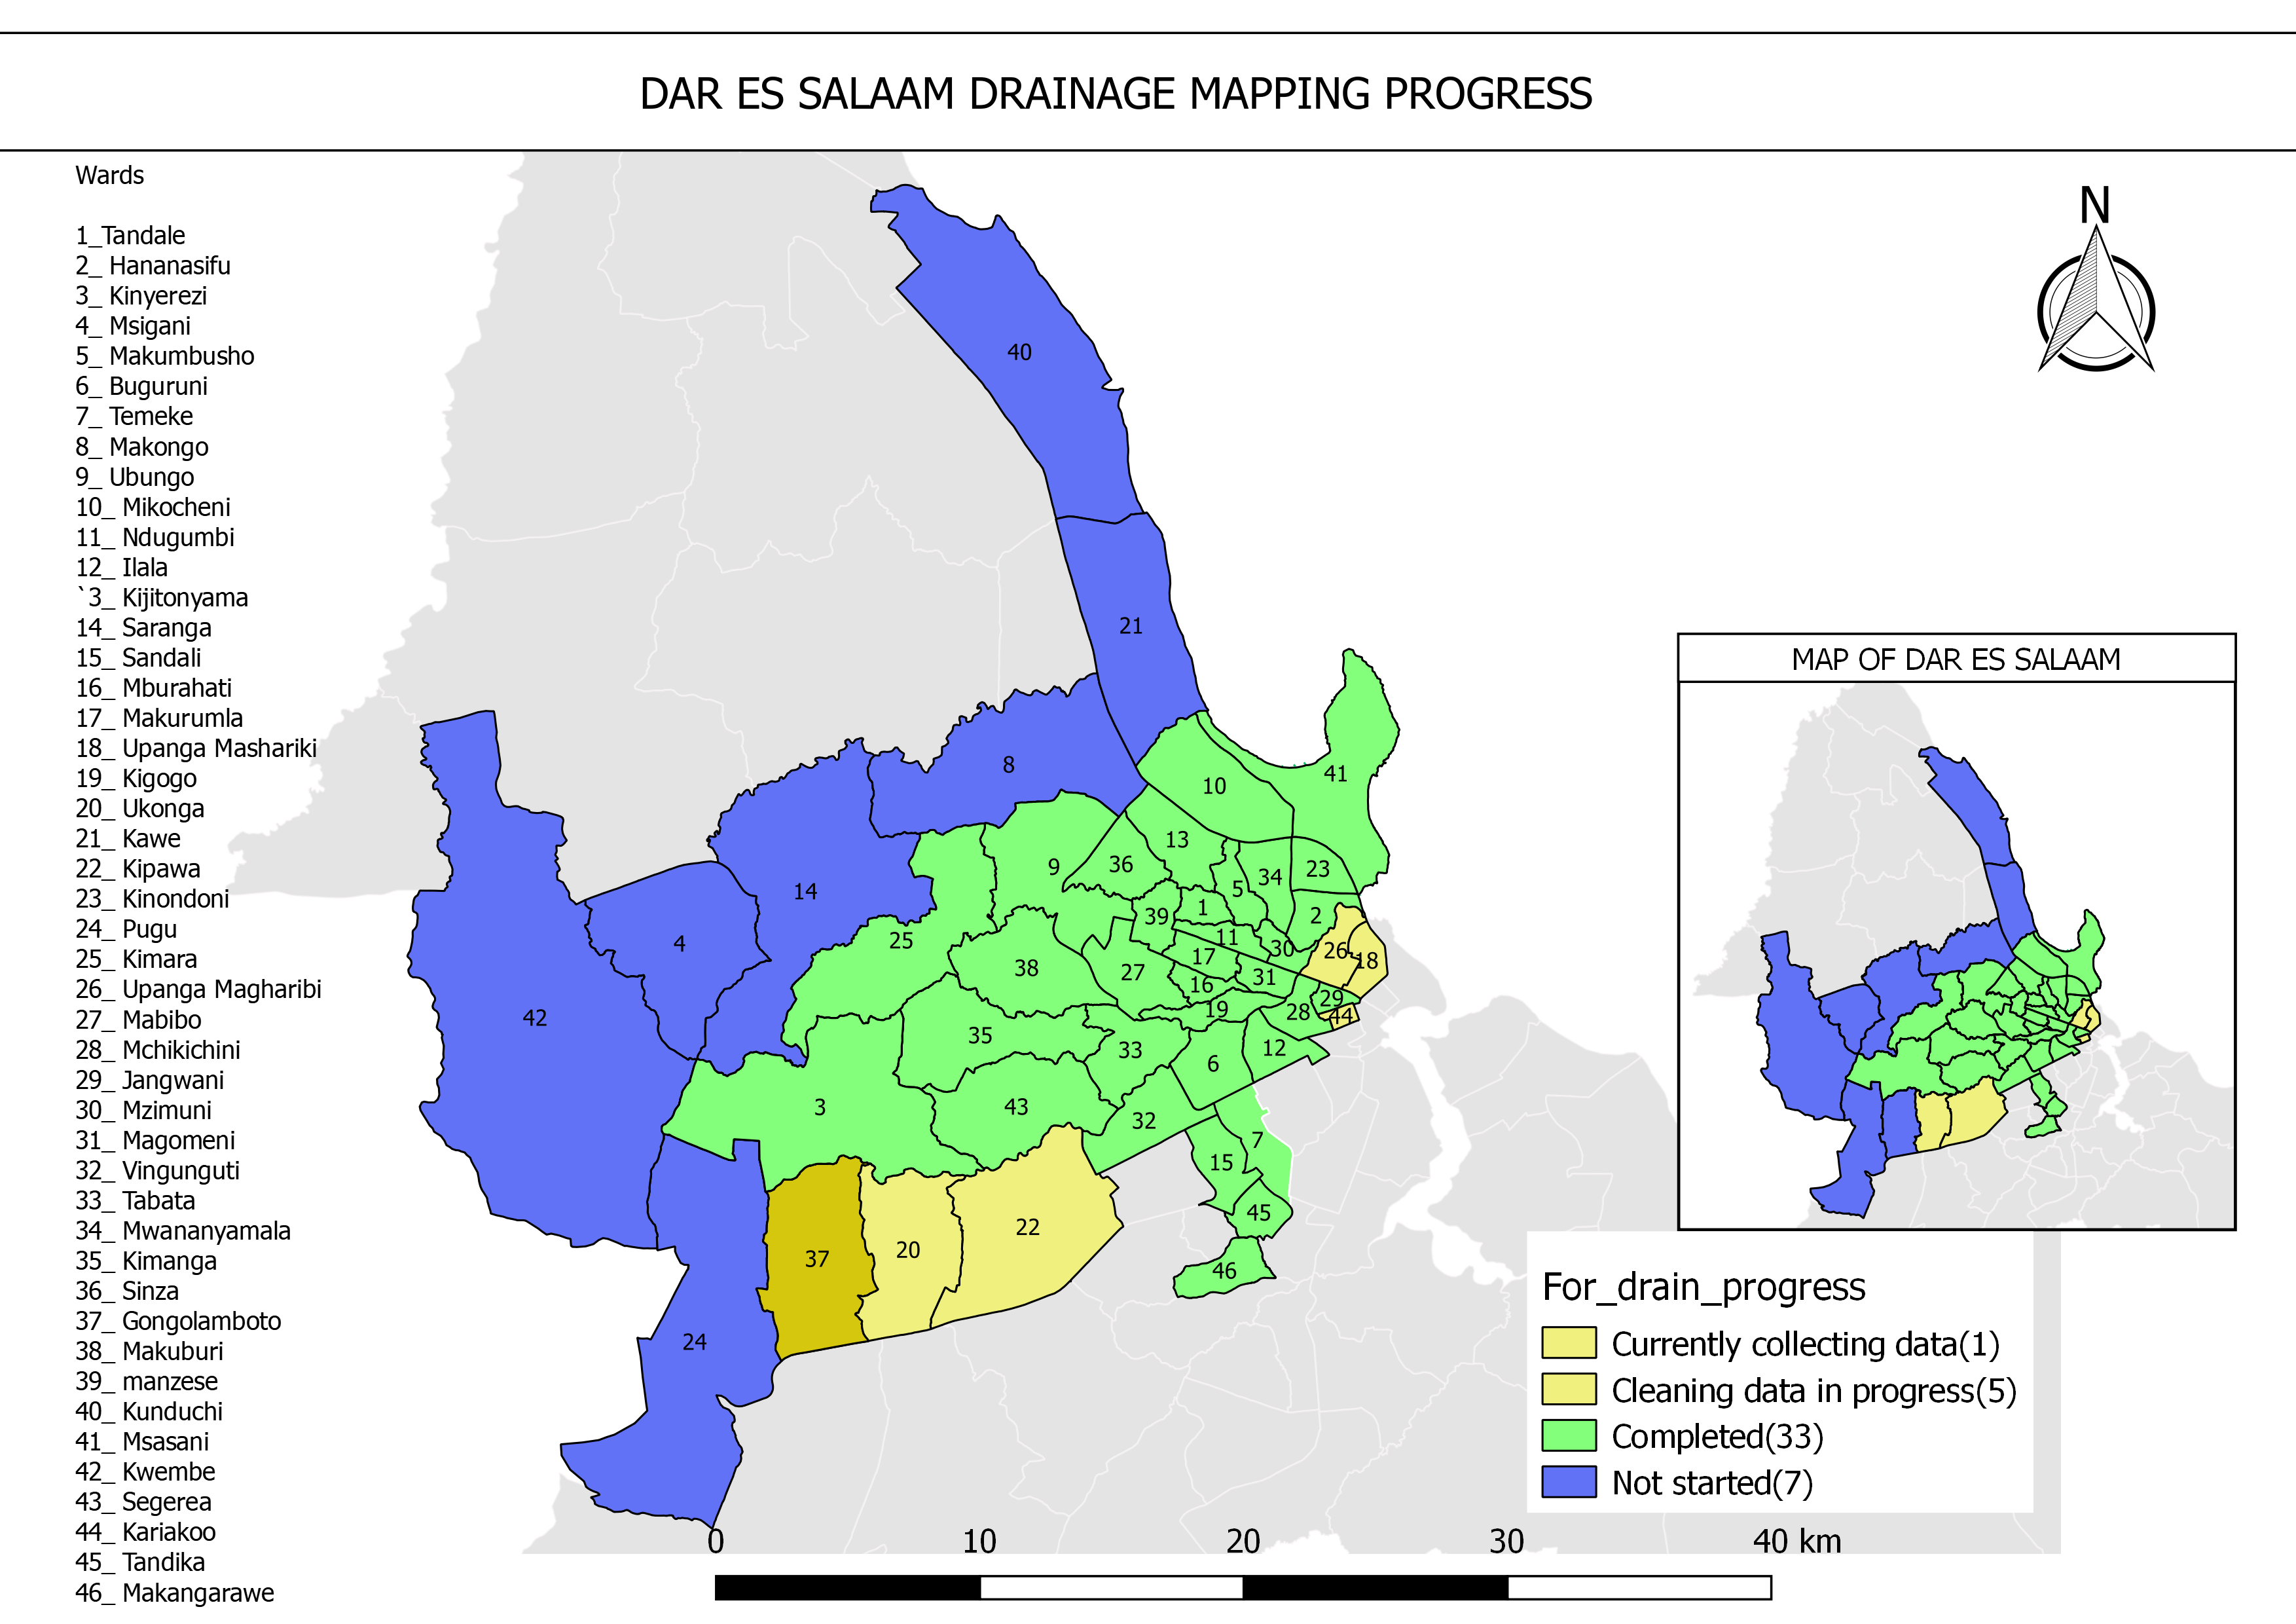
\includegraphics[width=1\textwidth]{images/Dar_drainage_mapping_progress.png}
\end{figure}

\subsubsection{Data Collection Methodology}

Drain points and segments data were traced using ODK Collect application. So far, drainage mapping has been completed in 38 wards of Dar es Salaam and 1 ward is still under cleaning process.

\subsubsection{Data Model}
\href{https://wiki.openstreetmap.org/wiki/Dar_es_Salaam/Ramani_Huria\#Drainage}{https://wiki.openstreetmap.org/wiki/Dar\_es\_Salaam/Ramani_Huria\#Drainage}

\subsubsection{Timeline}
August, 2017 and Ongoing

\subsubsection{Quality Assurance}

Drainage data is cleaned using QGIS with pre-installed template styles for the segments and points, a high resolution 2016 COWI imagery and in Hydro osm python model to ensure all drain segments and points are connected.

\subsubsection{Access}
\begin{itemize}
    \item \href{https://geonode.uhurulabs.org/layers/geonode\%3ADrain\%20Segments}{https://geonode.uhurulabs.org/layers/geonode\%3ADrain\%20Segments}
    \item \href{https://geonode.uhurulabs.org/layers/geonode\%3ADrain\%20Points}{https://geonode.uhurulabs.org/layers/geonode\%3ADrain\%20Points}
\end{itemize}

\subsubsection{Licencing}
\href{https://creativecommons.org/licenses/by/4.0/}{CC-BY 4.0}\footnote{\url{https://creativecommons.org/licenses/by/4.0/}}

\subsubsection{Statistics}
38 out of 44 wards of Dar es Salaam Ramani Huria prioritized wards completed
\begin{center}
\begin{tabular}{ |c|c|c| }
 \hline
 Number of Segments & 16207 \\ 
 \hline
 Number of Points & 12620 \\ 
 \hline
\end{tabular}
\end{center}

\subsubsection{Data Visualization}

\subsubsection{Use Case}
Development of a flood model and early warning systems

\subsubsection{Data Gap}

\subsubsection{Lessons Learned}

\newpage
\subsection{Soil Sediment Sampling}

Soil sediment profiles giving the soil particle sizes for surface and subsurface soils. Contains 643 soil sample points in a 2km by 2km grid covering Dar es Salaam.
Useful for erosion modeling, also potentially agriculture and building planning. 

\subsubsection{Spatial Extent}
Dar es Salaam and neighboring districts of Pwani region i.e. Bagamoyo, Kibaha and Kisarawe.

\begin{figure}[h]
  \color{RHgreen}\caption{A geo-referenced set of soil sediment profiles in Dar es Salaam and Pwani regions}
  \centering
  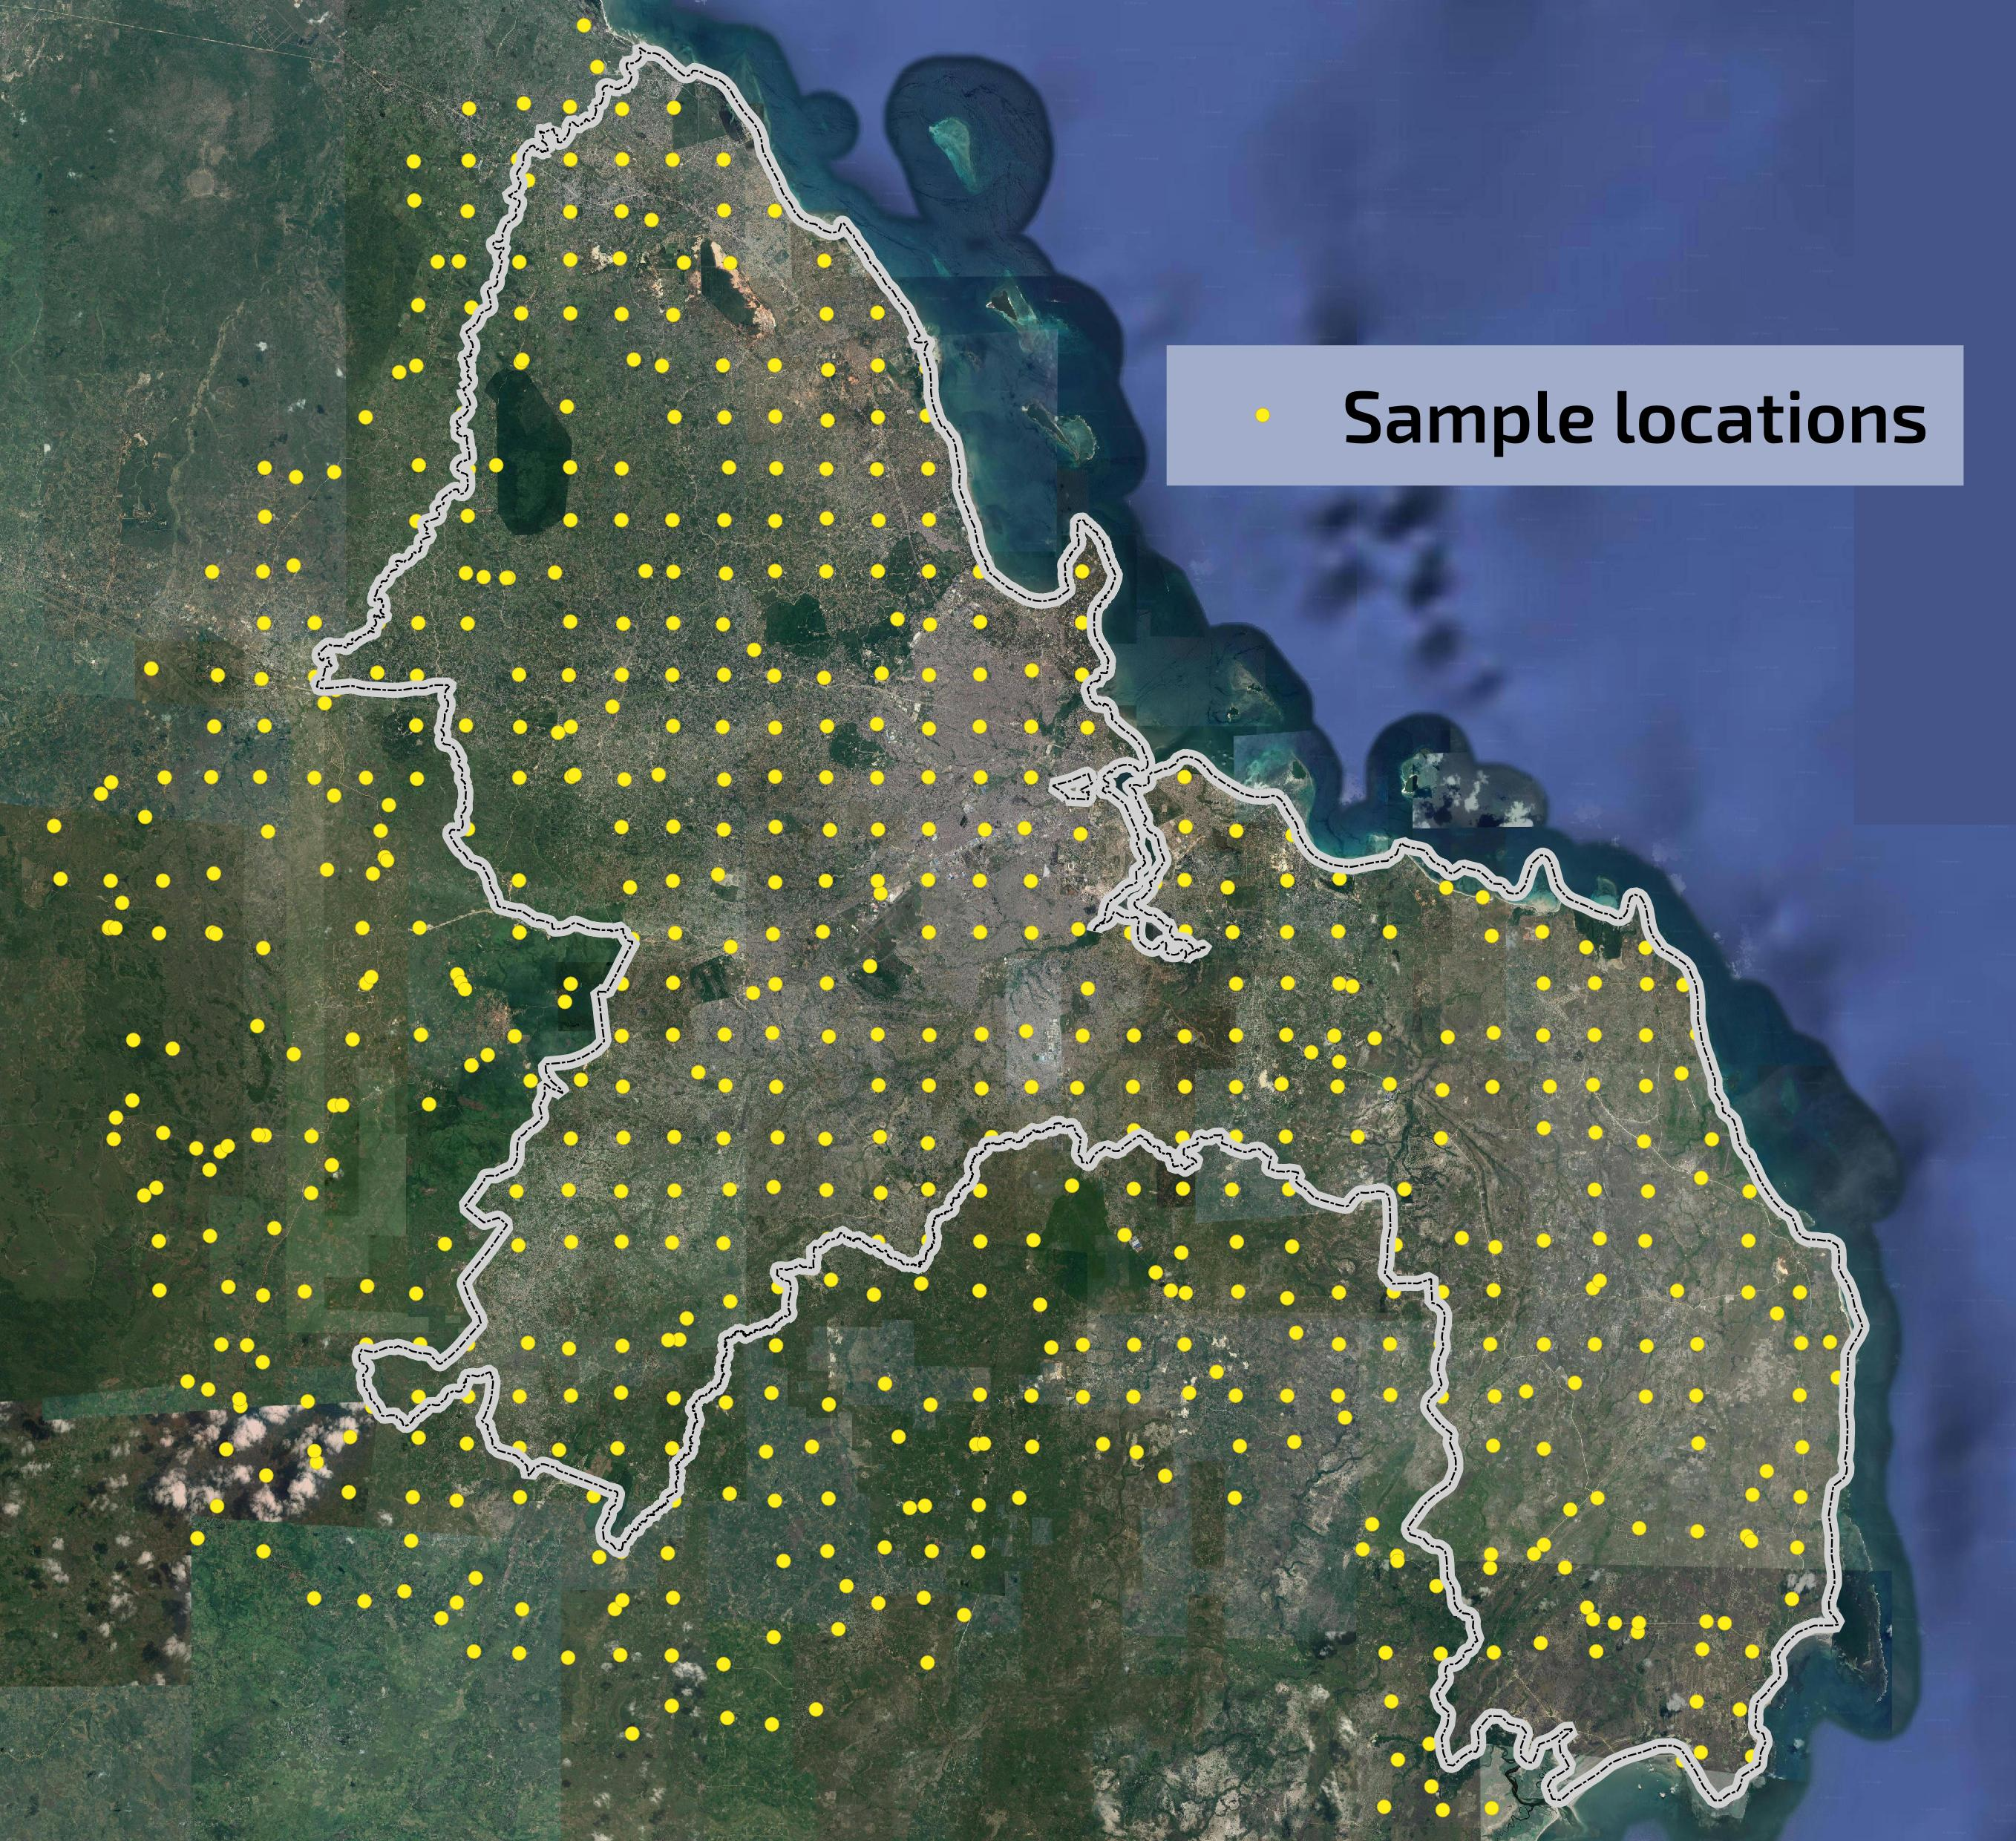
\includegraphics[width=0.8\textwidth]{images/soil_sample_locations.jpg}
\end{figure}

\subsubsection{Data Collection Methodology}

\begin{multicols}{2}
We created 2km by 2 km grid points. A set of data was recorded at each site using OpenDataKit’s Android application ODK Collect. Each field sampling team of two people carried the following equipment: trowel or small shovel, plastic “ziploc” bags with 1kg capacity, Android phone pre-loaded with ODK Collect---a separate maps and navigation application, maps.me---pre-loaded with the locations to be visited, first aid kit, marker pens, permission letter for the sampling activity from the municipal authorities and a tape measure.

We got training from a geo-morphologist and set up our own citizen-style lab to analyze the soil samples. The pair of samples—top and bottom—from each site was passed through a set of progressively finer-mesh sieves, resulting in nine separate fractions. Each fraction was weighed. The resulting measurements, which represent the proportion of each sediment particle size at each site, were
recorded.

The following materials were used: a set of metal sieves, scales, hand wash station and gloves, brush, cloth and towel for cleaning sieves, an Android phone with ODK Collect and sieving survey.
\end{multicols}

\subsubsection{Data Model}

\subsubsection{Timeline}
2018-10-11 to 2019-02-23

\subsubsection{Quality Assurance}

The quality control was done by  using ODK form to flag out any discrepancies such as negative masses or discrepancies in sums immediately.

\subsubsection{Access}
\href{https://geonode.uhurulabs.org/layers/geonode\%3A_2019_02_26_dar_soil_sampling_final_results_v1}{https://geonode.uhurulabs.org/layers/geonode\%3A20190226darsoilsamplingfinalresultsv1}

\subsubsection{Licencing}
CC-BY 4.0

\subsubsection{Statistics}
731 soil sample points created using a 2 km grid. 643 points sampled and sieved; 88 sample points were either inaccessible or hard to collect sample e.g. paved areas, military base.

\subsubsection{Data Visualization}
\begin{figure}[h]
  \color{RHgreen}\caption{A detail of the map showing the soil particle size in Dar es Salaam. The upward-facing histogram bars represent the top (surface) samples, and the downward-facing bars represent the bottom samples.}
  \centering
  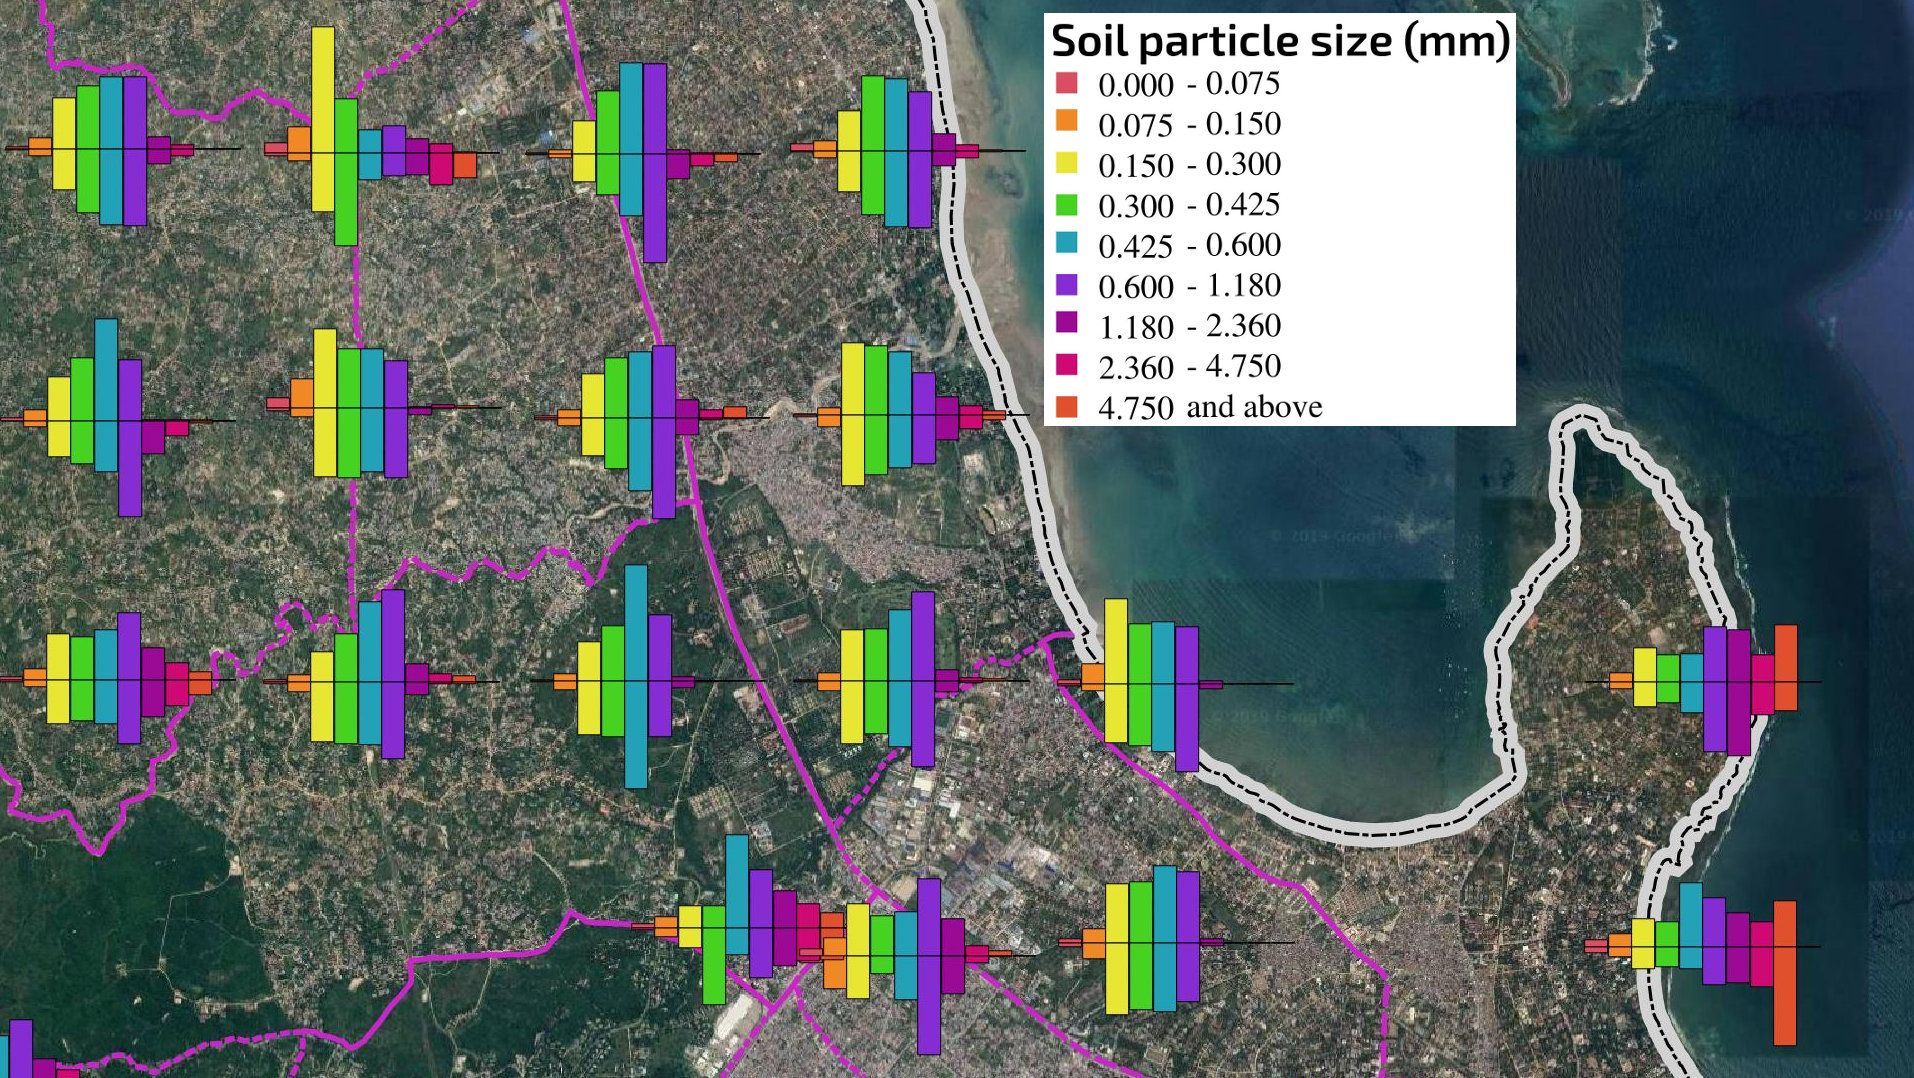
\includegraphics[width=1\textwidth]{soil_map_detail_peninsula_with_legend}
\end{figure}

\subsubsection{Use Case}
JBA  primarily intended for use this data for erosion modeling. The resulting dataset, a geo-referenced set of soil profiles, has been published as open data.

\subsubsection{Data Gap}
We have size of particles and maps but there is no data showing the chemical decomposition of soil.

\subsubsection{Lesson Learned}
Management of data is highly needed to avoid unnecessary cost.

\newpage

\subsection{Community Assets and Threats}

\begin{multicols}{2}
Flood risk identification on flood prone areas of the city by conducting a series of meetings with key people on specific subwards. Use of influential community members and leaders to identify assets (things that are important to the community), threats (things that the community "thinks" may flood if the hazard continues unabated) and issues that contribute to flooding in their subwards. This information can only be provided by the community itself since they understand their neighbourhoods better. The inventory covered  243 subwards in 49 wards of Dar es Salaam. 
\end{multicols}

\subsubsection{Spatial Extent}
The inventory covered  243 subwards in 49 wards of Dar es Salaam. 

\begin{figure}[h]
  \color{RHgreen}\caption{49 Wards covered during the community asset and threat mapping inventory}
  \centering
  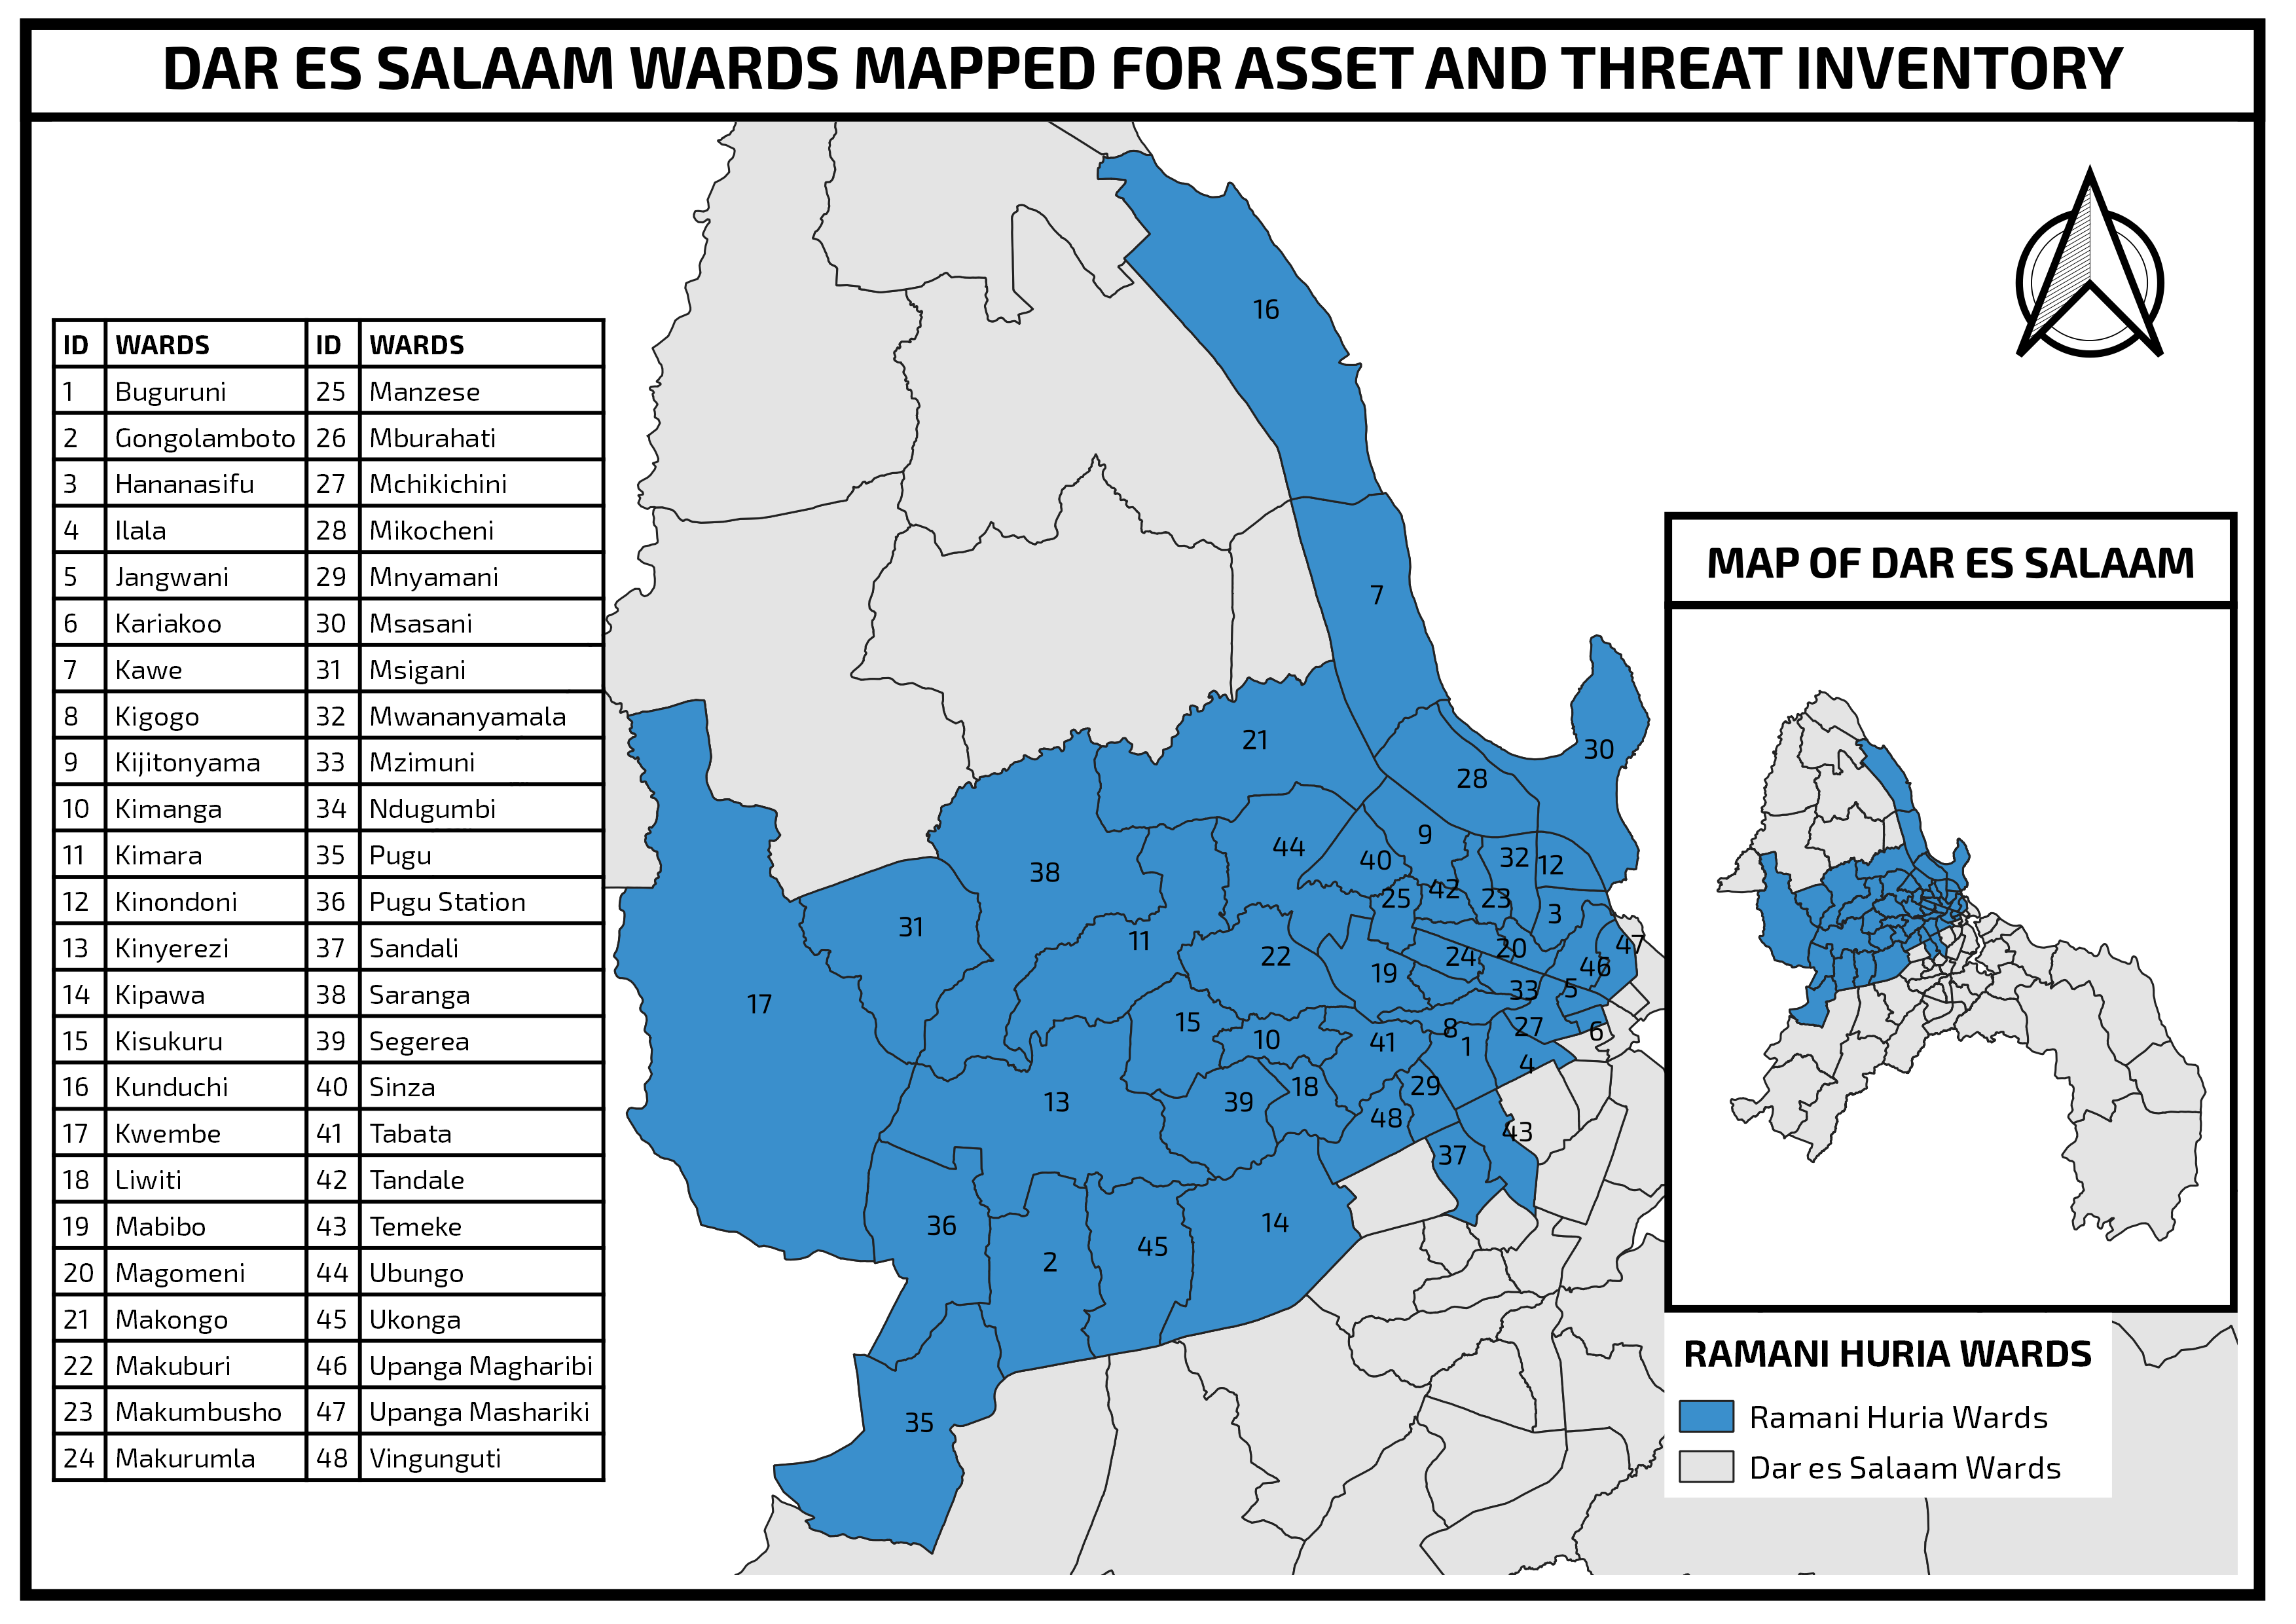
\includegraphics[width=0.8\textwidth]{images/asset_and_threat_wards.png}
\end{figure}

\subsubsection{Data Collection Methodology}

Setting up meetings with community leaders and influential people i.e. religious leaders in the specific wards. We first introduced how the data can help in reducing flooding, then ask them to identify and trace their boundaries on a map printed in A1 and point out assets and disaster threats in their neighbourhoods. We also printed satellite image maps of the respective subward to simplify identification of areas in their subwards.

Students worked in groups of six, visiting one subward at a time. After introductions were completed at the ward level, each subward mapping and data collection took approximately  4-5 days to complete. Threat and Asset inventory mappings were conducted in two different ways depending on whether the subward in question was mapped or unmapped. Student mappers split community members into three groups, each group guided by two students.

The discussion was based on three major key points:
\begin{enumerate}
    \item Assets (Important things in the subward)
    \item Assets under threats (incase the subward floods)
    \item Main causes of flood in the subward
\end{enumerate}

\subsubsection{Data Model}

\subsubsection{Timeline}
2018-06-08 to 2019-01-20

\subsubsection{Quality Assurance}
JOSM for editing buildings and roads and QGIS for field data analysis. Other sites are used for Quality Assurance for JOSM data are:
\begin{itemize}
    \item \href{https://qa.poole.ch/#}{QA}\footnote{\url{https://qa.poole.ch/#}}
    \item \href{http://osmose.openstreetmap.fr}{Osmose}\footnote{\url{http://osmose.openstreetmap.fr}}
    \item \href{http://keepright.at/}{KeepRight}\footnote{\url{http://keepright.at/}}
\end{itemize}

\subsubsection{Access}
\href{https://drive.google.com/drive/u/1/folders/1nW7luOI0A92GKi1vJtUJwt9P88OAzQ6h}{Dar es Salaam Asset and Threat Inventory}\footnote{\url{https://drive.google.com/drive/u/1/folders/1nW7luOI0A92GKi1vJtUJwt9P88OAzQ6h}}

\subsubsection{Licencing}
CC-BY 4.0

\subsubsection{Statistics}
A total of 5020 asset points were collected during the project. These include:
\begin{center}
\begin{tabular}{ |c|c|c| }
 \hline
 Assets at risk but not important & 28 \\ 
 \hline
 Evacuation centers & 42 \\ 
 \hline
 Important assets and at risk & 857 \\
 \hline
 Important assets but not at risk & 4093 \\
 \hline
 Roads and road names & 65868 \\
 \hline
 Landmarks & 1538 \\
 \hline
\end{tabular}
\end{center}

\subsubsection{Data Visualization}

\subsubsection{Use Case}
March, 2019 community flood response, creating resilience plans, mitigation measures through community mapping and impact assessment.

\subsubsection{Data Gap}
Out of 49 wards, historical flood extent was conducted in only 11 wards. There is a need of conducting flood extent in the remaining wards to create a better understanding of flooding.

\subsubsection{Lessons Learned}
Planning on paper vs actual fieldwork. We underestimated the time allocation in the work plan and number of training days which in turn resulted to a crappy work (maps and reports) leading to an  extension of time from October 2018 as the planned completion month to January 2019.

\medskip
We selected a few competent and committed students to re-do the maps and reports.


\newpage
\subsection{Buildings and Infrastructure}
\begin{multicols}{2}
Re-digitization of the city to update and improve the quality of already digitized layers using COWI imagery with 10cm resolution provided by the Ministry of Lands, Housing and Human Settlements. (Previously the city was digitized using either Bing, Mapbox or Digitalglobe which have lower resolutions compared to COWI imagery. So far the team has been able to digitize 28 out of 44 Ramani Huria wards. Namely Kisutu, Temeke, Vingunguti, Upanga Mashariki, Upanga Magharibi, Jangwani, Sandali, Kivukoni, Mwananyamala, Tabata, Kigogo, Kariakoo, Gerezani, Mchikichini, Hananasifu, Sinza, Kjitonyama, Magomeni, Tandale, Buguruni, Ilala, Keko, Mbagala, Mbagala kuu, Mabibo, Mchafukoge and Mzimuni. The wards digitized have a total of 299,691 buildings. This number includes new and existing buildings altogether.
\end{multicols}

\subsubsection{Spatial Extent}

\subsubsection{Data Collection Methodology}

Tracing and adjusting buildings from Mbtiles (offline imagery) which is updated and with higher resolution.

\subsubsection{Data Model}
\href{https://wiki.openstreetmap.org/wiki/Dar_es_Salaam/Ramani_Huria\#Buildings}{https://wiki.openstreetmap.org/wiki/Dar\_es\_Salaam/Ramani\_Huria\#Buildings}

\subsubsection{Timeline}
2018-08-24 to 2018-10-20

\subsubsection{Quality Assurance}
\begin{itemize}
    \item JOSM
    \item Tasking Manager
\end{itemize}

\subsubsection{Statistics}
28 wards have been re-digitized, though all 95 wards are digitized

\subsubsection{Data Visualization}


... 
\begin{figure}
  \begin{subfigure}[b]{0.5\textwidth}
    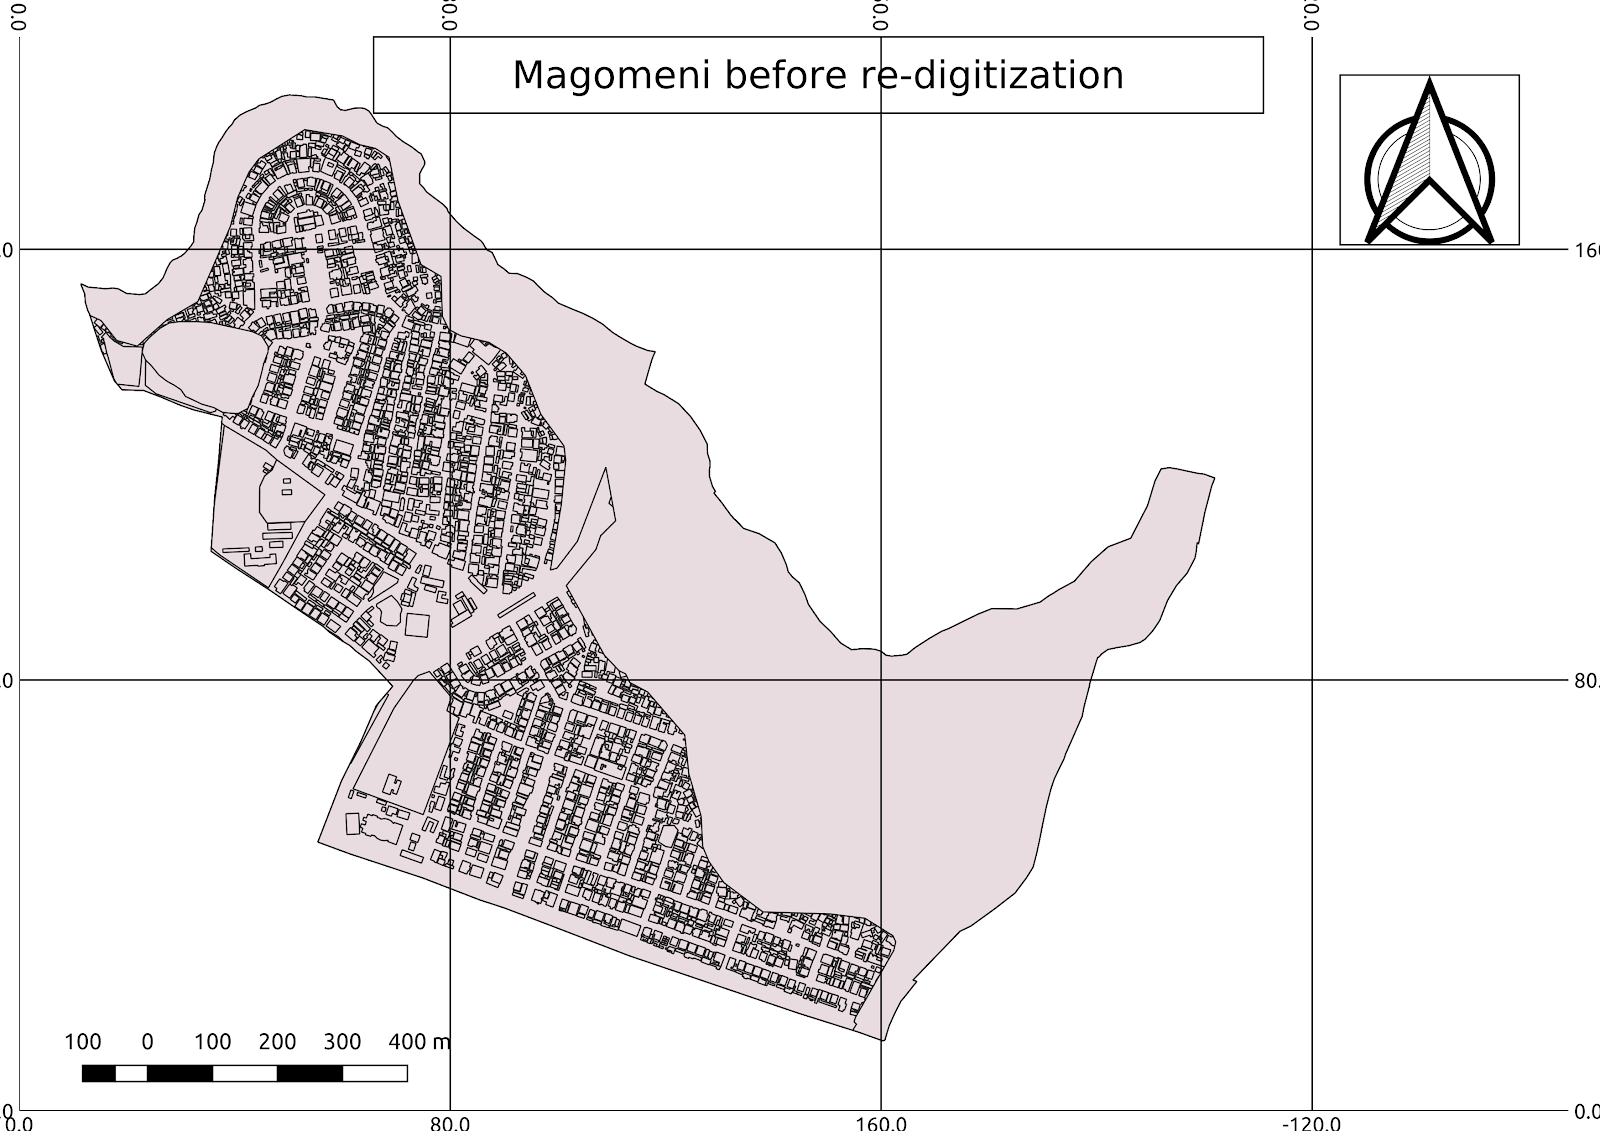
\includegraphics[width=\textwidth]{Magomeni_Before_Re-digitization.png}
   \color{RHgreen}\caption{Map showing Magomeni ward before re-digitization using UAV imagery}
    \label{fig:1}
  \end{subfigure}
  %
  \begin{subfigure}[b]{0.5\textwidth}
    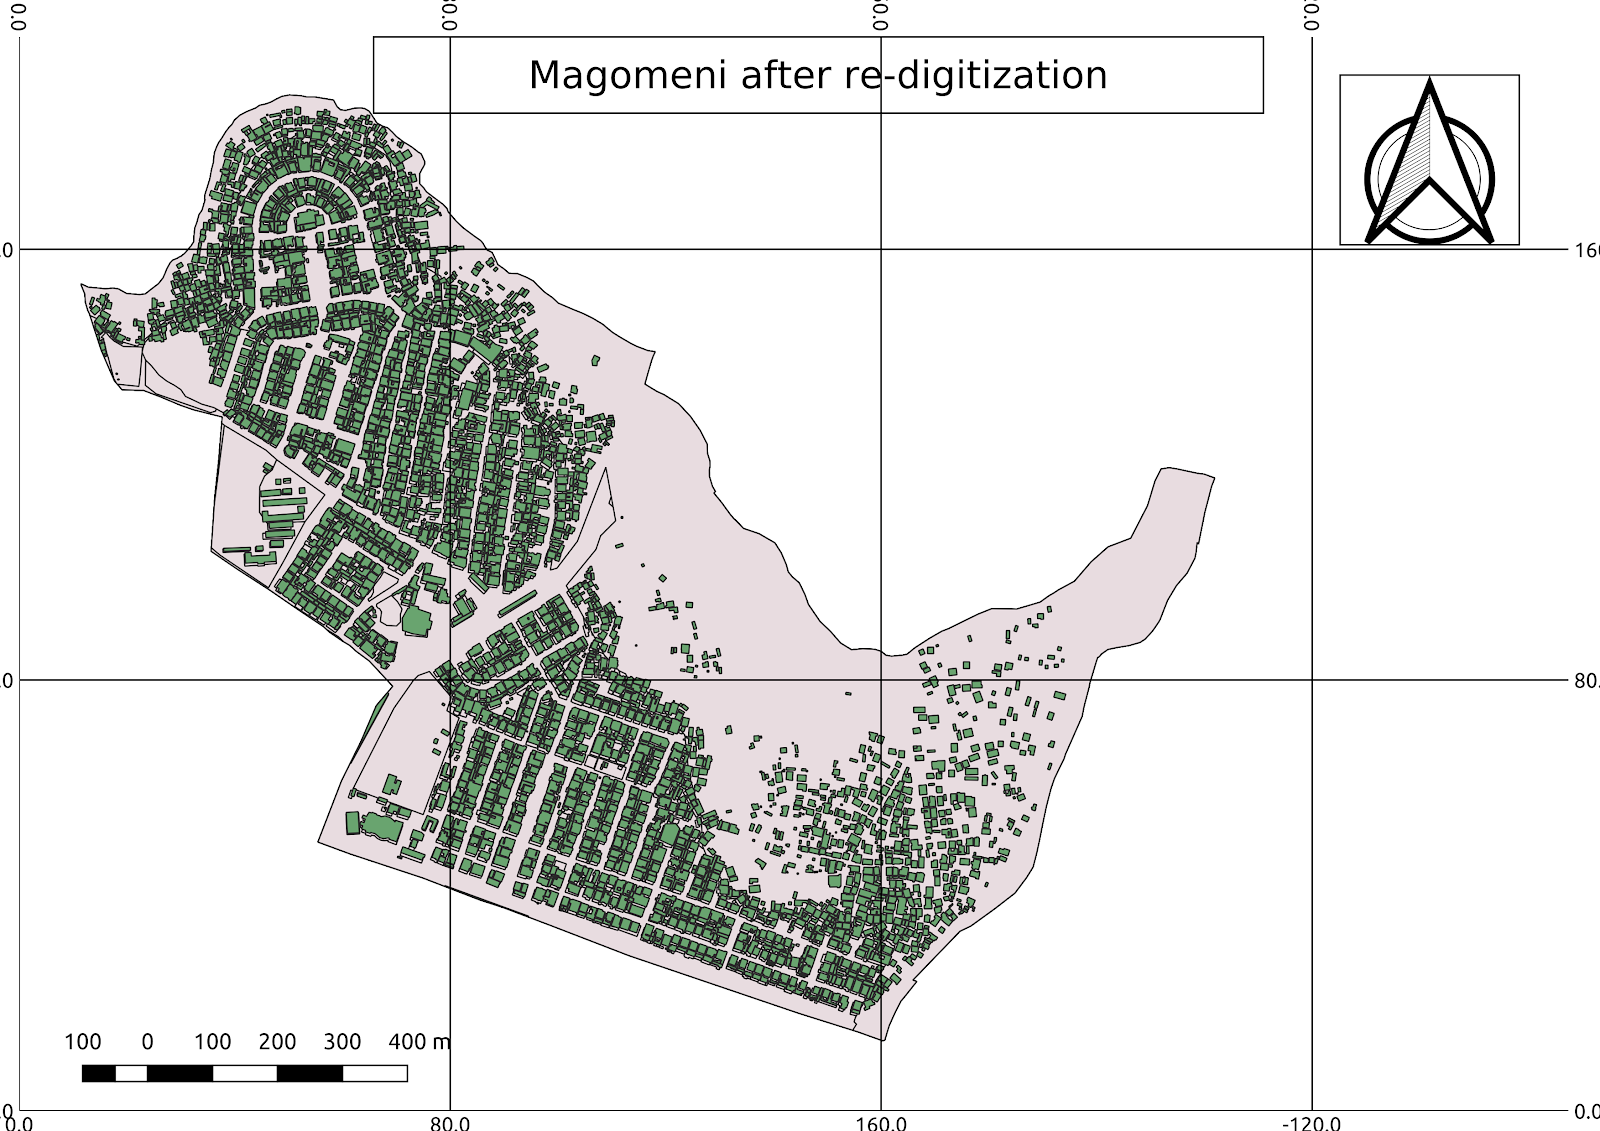
\includegraphics[width=\textwidth]{Magomeni_After_Re-digitization.png}
    \color{RHgreen}\caption{Map showing Magomeni ward after re-digitization using UAV imagery}
    \label{fig:2}
  \end{subfigure}
\end{figure}

\subsubsection{Use Case}
Apart from showing how buildings are arranged, the digitized data has been used in other Ramani Huria activities such as Green WastePro and Assets and Threat Mapping.

\subsubsection{Data Gap}

\subsubsection{Lessons Learned}

\newpage
\subsection{Administrative Divisions and Landmarks}
Hyperlocal boundaries are divisions within subwards regarded as political boundaries previously referred to as ten cell divisions as they were originally comprised of ten households.
Due to the increase in population, they comprise of 30 to 200 households and are administered by local leaders (wajumbe). Wajumbe are increasingly functioning as non-partisan public servants, often the first---in most cases---point of interaction between the government and citizens.

Given the rate of urbanization in Dar es Salaam, it is very difficult to locate people and their respective addresses due to the unplanned and informal nature of these communities. Using more granular boundaries however makes it easier to locate people and provide services more precisely. 

\subsubsection{Spatial Extent}
\begin{figure}[h]
  \color{RHgreen}\caption{Map showing Ramani Huria collaboration with Data Zetu hyper-local boundaries mapping}
  \centering
  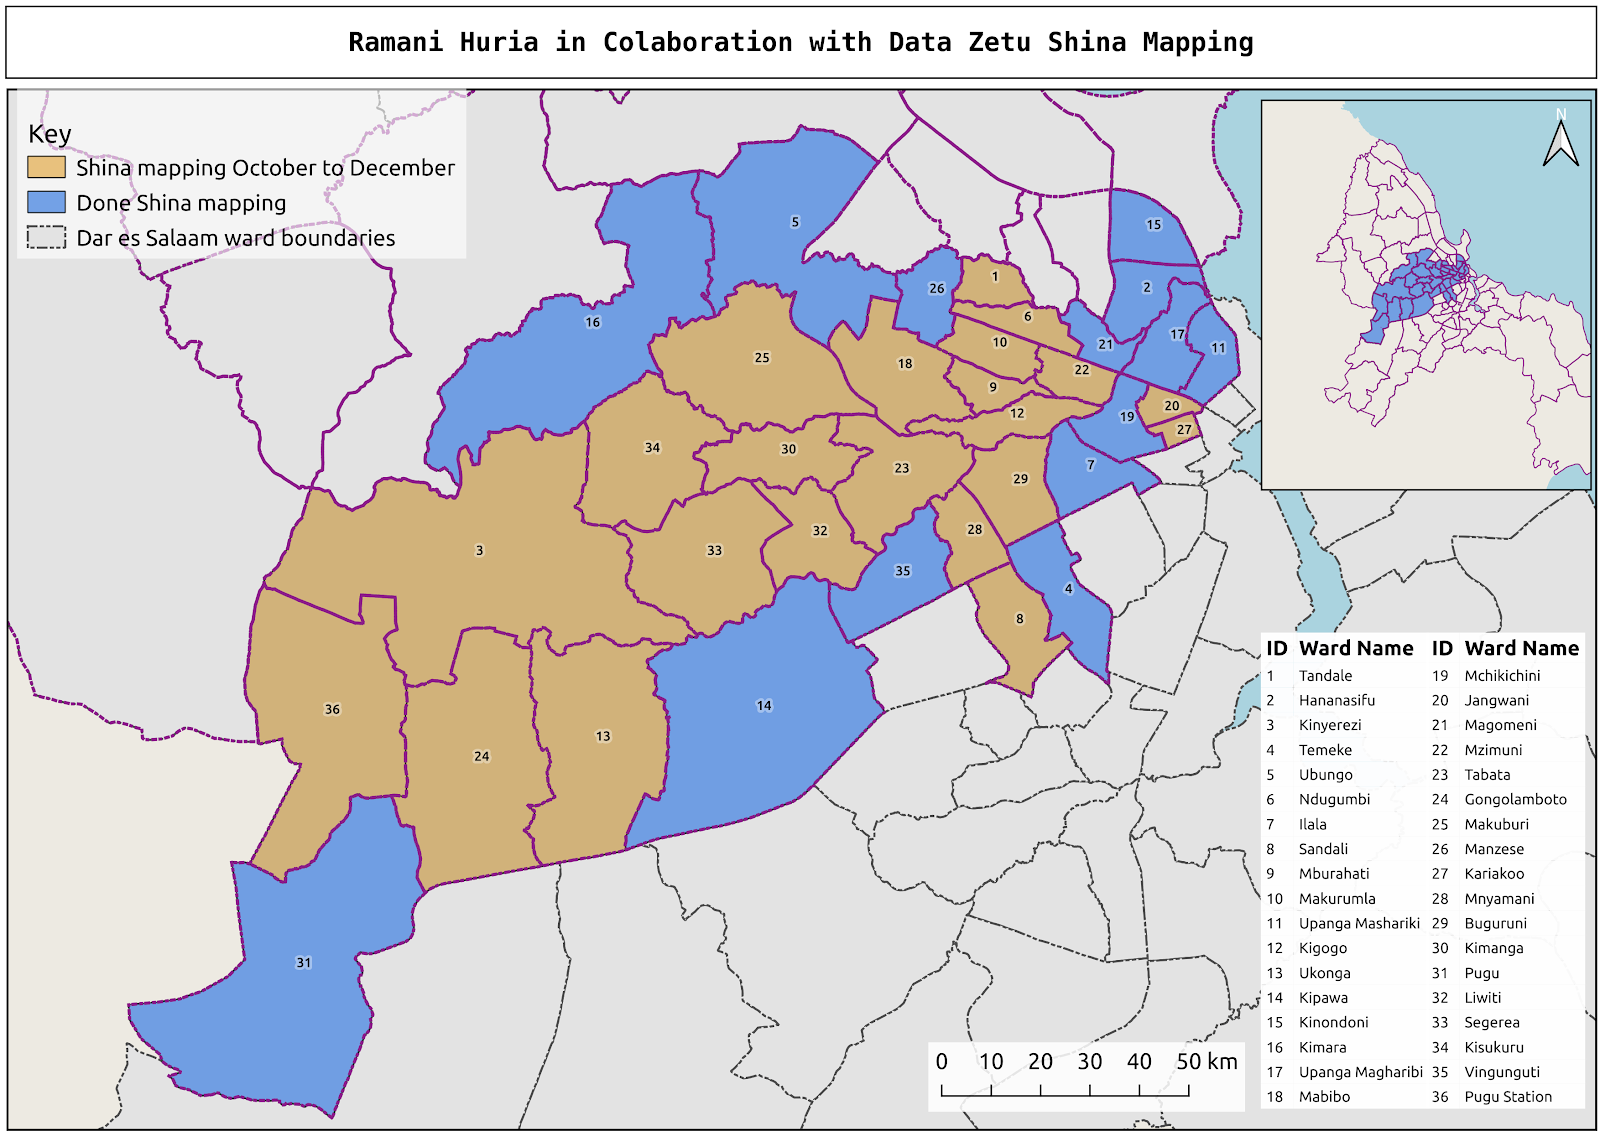
\includegraphics[width=0.8\textwidth]{images/RH_DZ_shina_boundaries.png}
\end{figure}

\subsubsection{Data Collection Methodology}

\subsubsection{Data Model}

\subsubsection{Timeline}
13/09/2018 to 24/12/2018

\subsubsection{Quality Assurance}
QGIS, Excel

\subsubsection{Statistics}
2612 local administrative boundaries mapped in 35 wards of Dar es Salaam

\subsubsection{Data Visualization}

\subsubsection{Use Case}
To find people’s address in Dar es Salaam, \href{https://www.hotosm.org/updates/piloting-tanzanias-first-patient-origin-tracking-system/}{Amana Hospital patient origin tracking system}\footnote{\url{https://www.hotosm.org/updates/piloting-tanzanias-first-patient-origin-tracking-system/}}

\subsubsection{Data Gap}
All hyperlocal boundaries have been cleaned and verified for map production except Mabibo subward. The team faced political misunderstandings among wajumbe as most of the hyperlocal boundaries overlapped among different political parties and made it difficult for the team to trace the boundaries.

\subsubsection{Lesson Learned}

\newpage
\subsection{Trash Mapping in Formal Settlement (Green WastePro Limited)}
Green WastePro Limited is a private company specialized in waste management with the aim to offer eco-friendly solutions in cleaning and waste management. They are mostly operate in formal settlements. The company needed digital methodology to obtain clients’ information including locations, clients contacts etc, so they can track clients and provide services accordingly.

\newpage
\subsection{Trash Mapping in Informal Settlement (Joshemi Company Limited)}

Joshemi Company Limited (JCL) is a company entitled by the Ilala Municipal to collect solid waste in Tabata ward with eight subwards therein. The system of collecting waste and doing cleanliness within the company was done locally by revenue collectors to collect service charges from the customers by using local tools.
\subsubsection {Spatial Extent}
2 pilot subwards (Msimbazi Magharibi and Msimbazi Mama) out of eight subwards in Tabata ward
\subsubsection{Methodology}
\subsubsection{Data Model}
\subsubsection{Timeline}
\subsubsection{Quality Control}
Google spreadsheet to fill in client information, JOSM for buildings, QGIS for client points
\subsubsection{Access}
\subsubsection{Licensing}
\subsubsection{Statistics}
20163 trash points collected in 2 subwards of Tabata ward
\subsubsection{Pictures}
\newpage
\subsubsection{Data Visualization}
\begin{figure}[h]
  \color{RHgreen}\caption{A map showing client distribution, houses and hyperlocal boundaries in Msimbazi Magharibi}
  \centering
 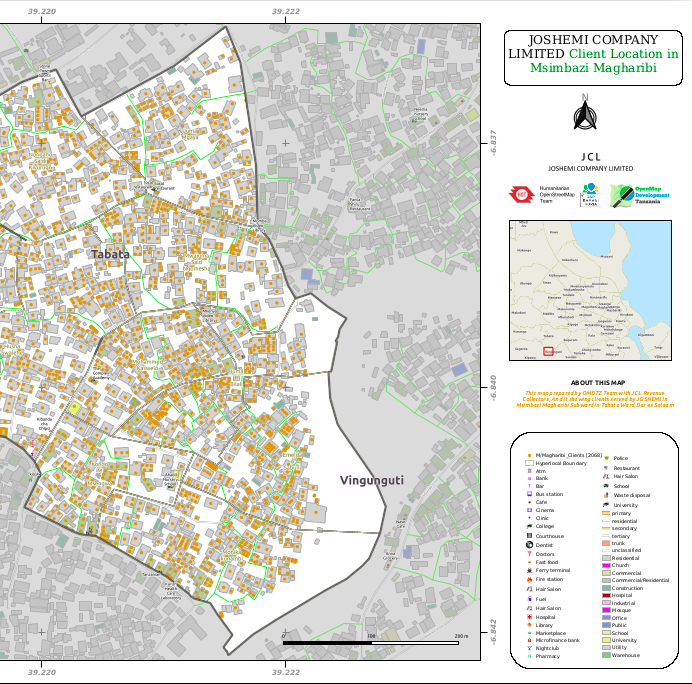
\includegraphics[width=0.8 \textwidth]{images/msimbazi_mama_data_viz.png}
\end{figure}


\subsubsection{Use Case}
\subsubsection{Data Gap}
\subsubsection{Lessons Learned}


\newpage
\subsection{Dar es Salaam Trash Data}

A collaboration between Nipe Fagio (“give me the broom” in Swahili), a civil society organization founded in 2013 and Ramani Huria that joined forces and mapped trash sites in Dar es Salaam. The trash mapping initiative was part and parcel of the large Let’s-Do-It-World campaign, a civic-led mass movement to clean up countries.
The mapped data helped to identify location of the areas with poorly managed waste materials, type and size of waste and clean up methods. This process helped ease cleaning the city on September 15th, 2018, a celebration of the world clean up day.

\subsubsection{Data Collection Methodology}
Using OpenDataKit to collect trash points in the city and filling out the survey on the type of waste (debris, glass, metal), and the size of trash (hand full, bag full, truckload, cart etc) to ease cleaning process.

Before field work, introduction letters were sent to ward officers so they can be informed and for mappers security in case there is any assistance needed from the ward office.

\subsubsection{Quality Assurance}
Some categories such as handful and bagful were far too small to be collected and sometimes confused the mappers therefore a decision to remove these points had to be made which dropped the number of points to approximately 9,000.

\newpage
\subsection{Community Flood Response Mapping}
\subsubsection{Summary}
As a response to heavy rainfall on March, 3rd, 2019, that resulted in heavy flooding in some wards of Dar es Salaam, the Ramani Huria team decided to conduct field mapping to engage affected communities with the aim of conducting a rapid assessment and producing impact maps.
\subsubsection{Spatial Extent}
3 majorly affected wards in Dar es Salaam with the March 3rd, 2019 rainfall (add map)

\newpage
\subsection{Historical Flood Extents}

Historical flood extent covered areas that are mostly affected by floods during rainy seasons. Households surveys were conducted to capture details in  subwards of the respective wards across the Msimbazi River rivers and streams that outflow to the main river.

\medskip

The information captured aimed to know whether the respondent had been affected by floods in the previous years, the flood depth and flood occurrence years---historical flood events. Individuals were asked to reflect on historical flood extents; therefore there is inherent subjectivity in their memories

\subsubsection{Spatial Extent}

\begin{figure}[h]
  \color{RHgreen}\caption{Map showing the flood extent mapping progress in Dar es Salaam}
  \centering
  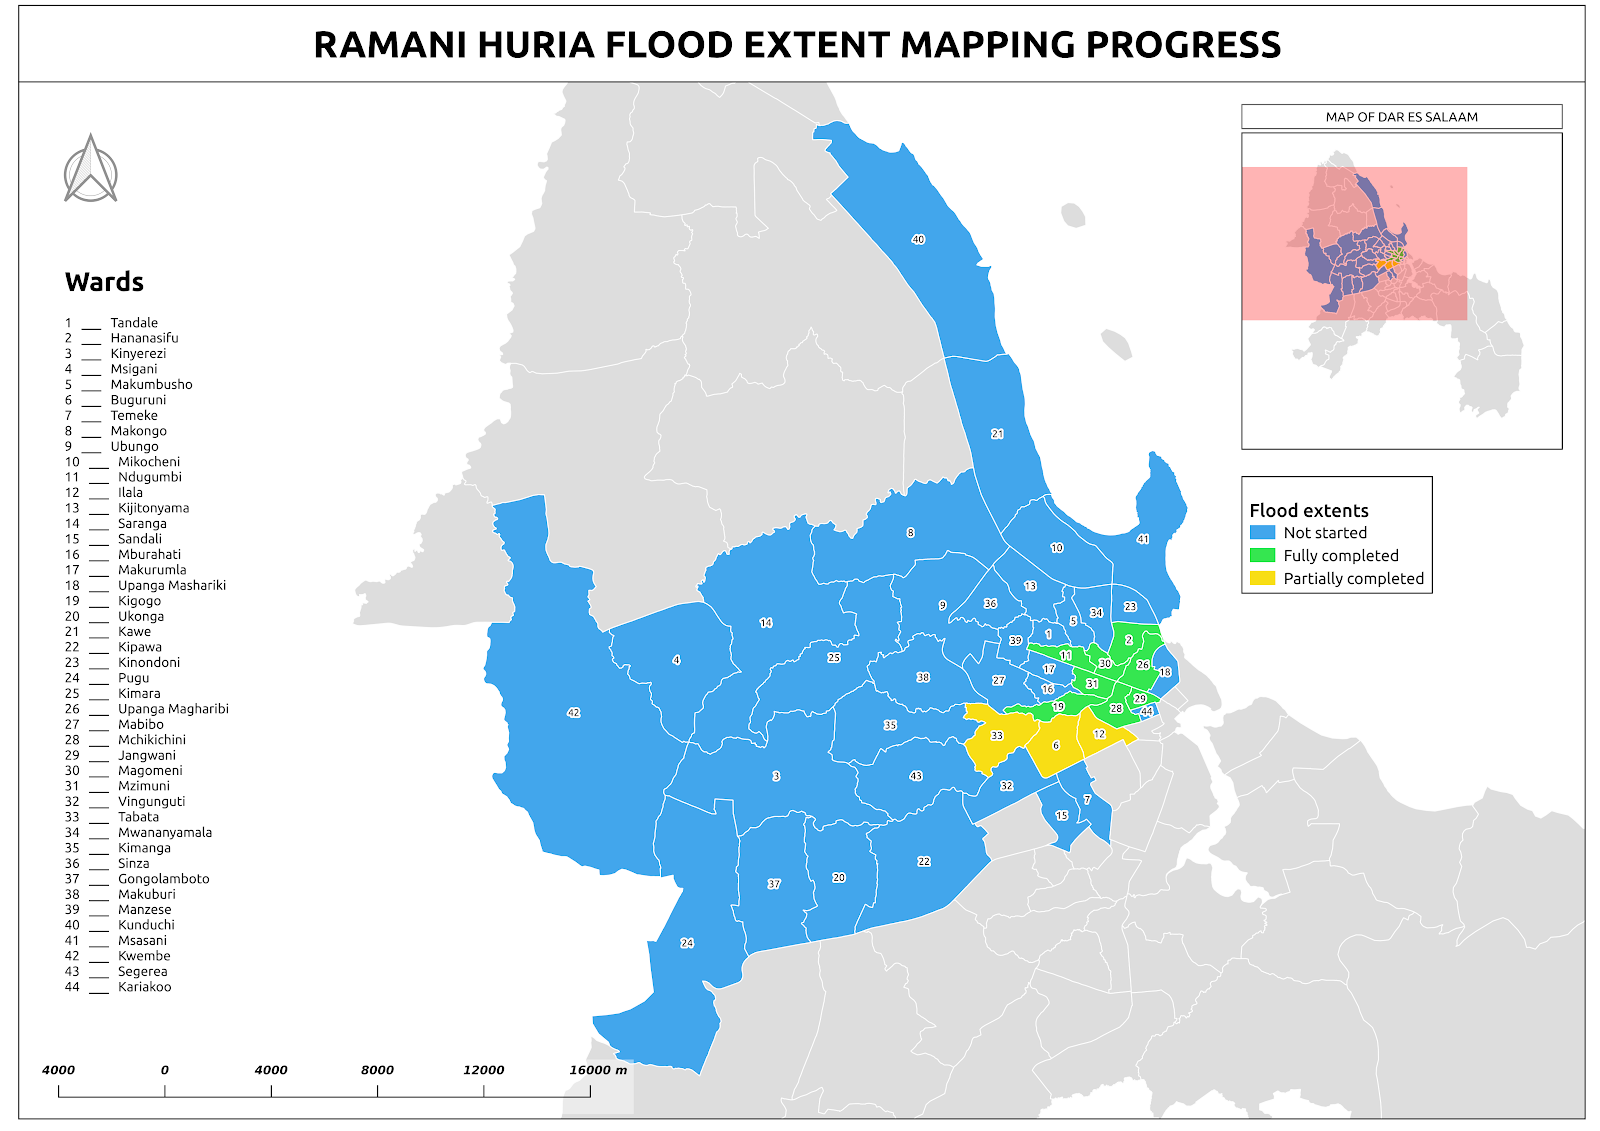
\includegraphics[width=0.8\textwidth]{images/RH_Flood_Extent_Progress.png}
\end{figure}

\subsubsection{Data Collection Methodology}

We met with people and asked them questions.

Sometimes they answered sensibly. Sometimes not. Sometimes we wrote down the answers. Sometimes not.

\subsubsection{Data Model}

\subsubsection{Timeline}
24/08/2017 to 12/04/2018

\subsubsection{Quality Assurance}
QGIS, Excel

\subsubsection{Statistics}
11 out of 44 prioritized Ramani Huria wards mapped, 30 000 household surveys

\subsubsection{Data Visualization}

\subsubsection{Use Case}

\subsubsection{Data Gap}
Individuals were asked to reflect on historical flood extents; therefore there is inherent subjectivity in their memories

\subsubsection{Lessons Learned}

\newpage
\section{Annexes}

\end{document}